% ==================================================
% CHAPTER 2: REQUIREMENTS AND PROCESS
% ==================================================

\chapter{Requirements and Development Process}
\label{ch:requirements}

\section{Stakeholders and Users}

\begin{itemize}
  \item \textbf{Readers} (students, developers, researchers): save pages and
  find them again. They are the primary users.
  \item \textbf{The maintainer}: deploys and operates the service, and
  receives problem reports.
  \item \textbf{External services}: Amazon Cognito (identity), Google Gemini
  (summaries) and Amazon SES (report email). MemoryLane depends on them but
  must keep working, with reduced features, when they fail.
\end{itemize}

\section{Use Cases}

Figure~\ref{fig:usecases} shows the use cases of the final system.

\begin{figure}[H]
\centering
\begin{tikzpicture}[node distance=3mm]
  % stick figure: \actor{x}{y}{label}
  \newcommand{\actor}[3]{%
    \draw[thick] (#1,#2+0.45) circle (2.2mm);
    \draw[thick] (#1,#2+0.23) -- (#1,#2-0.4);
    \draw[thick] (#1-0.35,#2) -- (#1+0.35,#2);
    \draw[thick] (#1,#2-0.4) -- (#1-0.25,#2-0.8);
    \draw[thick] (#1,#2-0.4) -- (#1+0.25,#2-0.8);
    \node[font=\small] at (#1,#2-1.1) {#3};}
  \actor{0}{-3.1}{Reader}
  \actor{7.5}{-5.4}{Maintainer}

  % extension use cases (left) and web-app use cases (right)
  \tikzset{usecase/.append style={minimum width=38mm, minimum height=8mm, font=\footnotesize}}
  \node[usecase] (signin)  at (-3.75, 0.0)  {Sign in (Google / email)};
  \node[usecase] (save)    at (-3.75,-1.25) {Save a page};
  \node[usecase] (auto)    at (-3.75,-2.5)  {Auto-capture pages};
  \node[usecase] (exclude) at (-3.75,-3.75) {Exclude a site};
  \node[usecase] (yt)      at (-3.75,-5.0)  {Save a YouTube video};
  \node[usecase] (undo)    at (-3.75,-6.25) {Undo / remove a save};
  \node[usecase] (search)  at (3.75, 0.0)  {Search by description};
  \node[usecase] (voice)   at (3.75,-1.25) {Search by voice};
  \node[usecase] (summ)    at (3.75,-2.5)  {Summarise a result};
  \node[usecase] (lib)     at (3.75,-3.75) {Browse the library};
  \node[usecase] (del)     at (3.75,-5.0)  {Delete a page / all data};
  \node[usecase] (report)  at (3.75,-6.25) {Report a problem};

  \begin{scope}[on background layer]
    \node[group, fill=gray!4, fit=(signin)(undo), inner sep=7pt] (extbox) {};
    \node[group, fill=gray!4, fit=(search)(report), inner sep=7pt] (webbox) {};
  \end{scope}
  \node[font=\small\bfseries, anchor=south] at (extbox.north) {Chrome extension};
  \node[font=\small\bfseries, anchor=south] at (webbox.north) {Web app};

  \foreach \u in {signin,save,auto,exclude,yt,undo}
    \draw (-0.35,-3.1) -- (\u.east);
  \foreach \u in {search,voice,summ,lib,del,report}
    \draw (0.35,-3.1) -- (\u.west);
  \draw (7.15,-5.4) -- (report.east);
  \draw[dashed,->] (voice) -- node[lbl, right] {$\ll$extend$\gg$} (search);
\end{tikzpicture}
\caption{Use-case diagram of MemoryLane}
\label{fig:usecases}
\end{figure}

\section{Functional Requirements}

\begin{longtable}{>{\ttfamily}p{0.09\textwidth} p{0.6\textwidth} p{0.18\textwidth}}
\toprule
\textrm{\textbf{ID}} & \textbf{Requirement} & \textbf{Status} \\
\midrule
\endhead
FR-01 & Users sign in with Google or email and password; a Google and an email sign-in with the same verified email share one library. & Done \\
FR-02 & The extension saves the current page in one click, confirms it, and offers undo. & Done \\
FR-03 & Optional automatic capture saves only pages the user has read and that look like content, and never private pages (email, banking, private apps, account areas). & Done \\
FR-04 & Users can exclude sites from automatic capture and see and remove the day's automatic saves. & Done \\
FR-05 & YouTube videos are saved through their captions, with description and channel. & Done \\
FR-06 & Saving the same page again updates one entry; addresses that differ only in tracking parameters, \texttt{www.} or fragments are the same page. & Done \\
FR-07 & Users search with a natural-language description, by typing or by voice, and get up to ten pages with snippets. & Done \\
FR-08 & Queries that name a site, a time or a URL rank matching pages higher. & Done \\
FR-09 & Each result can be summarised on demand. & Done \\
FR-10 & Users browse their library newest first, delete pages with undo, and delete all their data. & Done \\
FR-11 & Users report a problem from the website or the extension; the report is emailed to the maintainer. & Done \\
FR-12 & A public health endpoint reports the state of Solr, the model and Gemini. & Done \\
\bottomrule
\caption{Functional requirements}
\label{tab:fr}
\end{longtable}

\section{Non-Functional Requirements}

\begin{table}[H]
\centering
\small
\begin{tabularx}{\textwidth}{>{\raggedright\arraybackslash}p{0.2\textwidth} L L}
\toprule
\textbf{Quality} & \textbf{Requirement} & \textbf{How it is met} \\
\midrule
Privacy & No user can see or change another user's pages; sensitive pages are never auto-saved; logs hold no URLs or queries & User filter inside the Solr client; isolation tests; two-stage capture rules; log filters \\
Security & Authenticated API; no secrets in the browser & Cognito PKCE, RS256 token checks, CSP, HTTPS with HSTS, rate limits \\
Performance & Search answers in well under a second & $\approx$75\,ms median in-process search; concurrent BM25 and KNN \\
Relevance & The right page is usually first & Hit@1 0.71, MRR@10 0.79 on SciFact (Chapter~\ref{ch:evaluation}) \\
Availability & Survives a reboot; degrades instead of failing & Restart policies, health checks; summaries and reports optional \\
Maintainability & Changes are safe and explained & 551 tests, CI, decision records, documentation site \\
Usability & Usable with keyboard and on phones & Keyboard shortcuts, responsive layout, voice input \\
Cost & Runs on one small server & One \texttt{c7i-flex.large} instance \\
\bottomrule
\end{tabularx}
\caption{Non-functional requirements}
\label{tab:nfr}
\end{table}

\section{Development Process}

MemoryLane was built \textbf{iteratively and incrementally}
\cite{sommerville2016se}: each iteration delivered a working system, which
was used, measured and then improved. Work was tracked in Git on GitHub, with
feature branches for larger changes (for example
\texttt{feature/library-map}) and 86 commits over four months.

\begin{figure}[H]
\centering
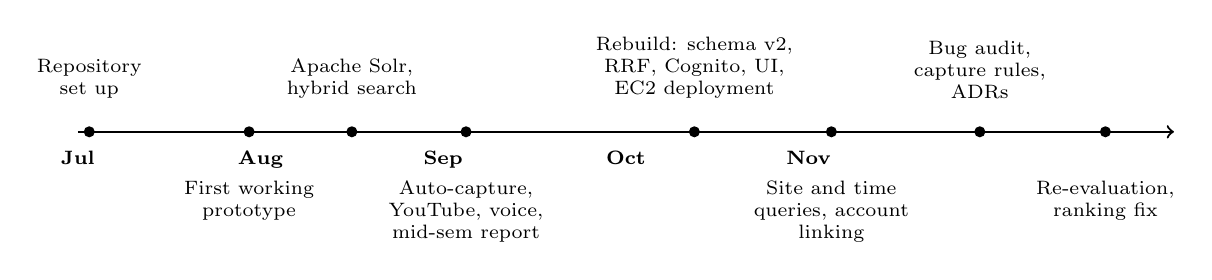
\begin{tikzpicture}[x=1.45cm]
  \draw[thick,->] (0,0) -- (9.6,0);
  \foreach \x/\m in {0/Jul, 1.6/Aug, 3.2/Sep, 4.8/Oct, 6.4/Nov}
    \node[font=\scriptsize\bfseries, below] at (\x,-0.12) {\m};
  \foreach \x in {0.1,1.5,2.4,3.4,5.4,6.6,7.9,9.0}
    \fill (\x,0) circle (2pt);
  \node[font=\scriptsize, align=center, above=3mm] at (0.1,0) {Repository\\ set up};
  \node[font=\scriptsize, align=center, below=5mm] at (1.5,0) {First working\\ prototype};
  \node[font=\scriptsize, align=center, above=3mm] at (2.4,0) {Apache Solr,\\ hybrid search};
  \node[font=\scriptsize, align=center, below=5mm] at (3.4,0) {Auto-capture,\\ YouTube, voice,\\ mid-sem report};
  \node[font=\scriptsize, align=center, above=3mm] at (5.4,0) {Rebuild: schema v2,\\ RRF, Cognito, UI,\\ EC2 deployment};
  \node[font=\scriptsize, align=center, below=5mm] at (6.6,0) {Site and time\\ queries, account\\ linking};
  \node[font=\scriptsize, align=center, above=3mm] at (7.9,0) {Bug audit,\\ capture rules,\\ ADRs};
  \node[font=\scriptsize, align=center, below=5mm] at (9.0,0) {Re-evaluation,\\ ranking fix};
\end{tikzpicture}
\caption{Project timeline, July--November 2026}
\label{fig:timeline}
\end{figure}

The October rebuild was planned as seven phases, each committed and tested
separately: query-side retrieval improvements, bug fixes, a new ingestion
pipeline and schema, authentication and multi-user scoping, a web redesign,
an extension redesign, and deployment with Docker Compose and Caddy. After
the system went live, real use drove the remaining work: an audit of
reported bugs, stricter automatic capture after an inbox was captured by an
outdated extension, and a second evaluation that uncovered a ranking defect
(Section~\ref{sec:bonus}).

Every significant choice was written down as an \textbf{architecture
decision record} (ADR) \cite{nygard2011adr}, giving the context, the
decision, the alternatives and the consequences (Table~\ref{tab:adrs}).
Features that did not earn their place were removed rather than kept, and
their removal was recorded too.
